\section{SECCIÓN 6. TESTS}
\textit{Identificar todas las demás pruebas no incluidas en la verificación y validación y establecer los métodos utilizados. Describir cualquier técnica o método de prueba que se pueda utilizar para detectar errores, desarrollar conjuntos de datos de prueba y monitorear los recursos del sistema informático.}

La actividad de prueba del proyecto incluye pruebas a nivel de unidad, pruebas de integración (a nivel de Unidad y CI/HWCI), pruebas de rendimiento (Pruebas de Calificación de CI) y pruebas de aceptación (Pruebas de Calificación del Sistema). La Figura 6-1 proporciona el Diagrama de Flujo del Proceso de Prueba. SQA auditará las actividades de prueba según lo definido en la referencia (e), y verificará que el software y la documentación de prueba estén sujetos al control de gestión de configuración. SQA presenciará las pruebas y verificará que los resultados de las pruebas se registren y evalúen. SQA coordinará el mantenimiento de los registros de Informes de Problemas/Cambios (P/CR), a veces llamados Informes de Problemas de Software (STR), con SCM y verificará que los cambios de software se controlen según la referencia (e). SQA presenciará las pruebas de regresión resultantes de P/CR o STR para verificar la efectividad de la corrección.

\begin{figure}[H]
\centering
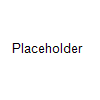
\includegraphics[width=0.8\textwidth]{images/imagen3.png}
\caption{Diagrama de Flujo del Proceso de Prueba}
\label{fig:testflow}
\end{figure}

\subsection{6.1 SISTEMA BAJO PRUEBA Y NIVELES DE PRUEBA}

El sistema bajo prueba (SUT) es una Galería de Imágenes Segura desarrollada con Spring Boot 4.0.6 sobre Java 21, frontend React 18 con Vite y persistencia en PostgreSQL. Su característica diferenciadora es la detección de contenido oculto mediante análisis de esteganografía (anomalías EOF, firmas embebidas y metadatos EXIF), con cuarentena de archivos sospechosos y un panel de supervisor para auditoría.

Las pruebas se organizan en los siguientes niveles:

\begin{table}[H]
\centering
\caption{Niveles de prueba y su implementación}
\label{tab:niveles}
\begin{tabular}{|p{3.2cm}|p{5.3cm}|p{5.3cm}|}
\hline
\textbf{NIVEL} & \textbf{ALCANCE} & \textbf{IMPLEMENTACIÓN} \\
\hline
Unitario & Lógica de detección de esteganografía y validación de archivos & \texttt{FileStorageServiceTest} (JUnit 5) \\
\hline
Persistencia & Consultas y estados de las entidades \texttt{Image} y \texttt{Album} & \texttt{ImageRepositoryTest}, \texttt{AlbumSanitizationJpaTest} (\texttt{@DataJpaTest} sobre H2) \\
\hline
Integración & Endpoints REST con cadena de seguridad y control de acceso & \texttt{SupervisorControllerTest}, \texttt{SupervisorPanelAuditTest}, \texttt{XssSanitizationTest}, \texttt{AlbumAuthorizationTest} (\texttt{MockMvc}) \\
\hline
Seguridad & Sanitización XSS, autorización por rol, path traversal y CSRF & Distribuido entre las clases de integración \\
\hline
Sistema (E2E) & Flujos críticos del frontend & Cypress (\texttt{quarantine-harmless}, \texttt{quarantine-harmful}) \\
\hline
Estático & Deuda técnica, code smells y vulnerabilidades de código & SonarQube, Qlty, \texttt{npm audit} \\
\hline
Cobertura & Medición cuantitativa de la cobertura alcanzada & JaCoCo \\
\hline
\end{tabular}
\end{table}

\subsection{6.2 MATRIZ DE TRAZABILIDAD}

La siguiente matriz relaciona cada requisito funcional con los casos de prueba que lo verifican.

\begin{longtable}{|p{2.2cm}|p{1.8cm}|p{10cm}|}
\hline
\textbf{REQUISITO} & \textbf{CASO} & \textbf{DEFINICIÓN DEL CASO DE PRUEBA} \\
\hline
\endfirsthead
\hline
\textbf{REQUISITO} & \textbf{CASO} & \textbf{DEFINICIÓN DEL CASO DE PRUEBA} \\
\hline
\endhead
\multirow{5}{*}{\parbox{2cm}{RF-01\\Registro y Autenticación Segura}}
 & CP01 & Un usuario intenta registrarse usando datos válidos \\
\cline{2-3}
 & CP02 & Un usuario intenta registrarse usando datos incorrectos o inválidos \\
\cline{2-3}
 & CP03 & Un usuario con cuenta intenta iniciar sesión con credenciales válidas \\
\cline{2-3}
 & CP04 & Un usuario con cuenta intenta iniciar sesión con credenciales inválidas \\
\cline{2-3}
 & CP05 & Un usuario intenta ingresar repetidamente con credenciales inválidas \\
\hline
\multirow{5}{*}{\parbox{2cm}{RF-02\\Control de Acceso y Sesión}}
 & CP06 & Un usuario con rol USER intenta acceder a funcionalidades exclusivas del SUPERVISOR \\
\cline{2-3}
 & CP07 & Un usuario con rol SUPERVISOR accede al panel de administración \\
\cline{2-3}
 & CP08 & Un usuario no autenticado intenta acceder a un recurso protegido \\
\cline{2-3}
 & CP09 & Un JWT expirado es enviado al sistema \\
\cline{2-3}
 & CP10 & Se solicita un nuevo Access Token mediante un Refresh Token válido \\
\hline
\multirow{7}{*}{\parbox{2cm}{RF-03\\Detección de Esteganografía}}
 & CP11 & Se analiza un archivo con contenido oculto no dañino (anomalía EOF) \\
\cline{2-3}
 & CP12 & Se analiza un archivo con datos post-EOF menores al umbral de anomalía \\
\cline{2-3}
 & CP13 & Se analiza un archivo limpio sin datos ocultos \\
\cline{2-3}
 & CP14 & Se solicita el reporte de esteganografía de un archivo con hallazgo \\
\cline{2-3}
 & CP15 & Se analiza un archivo con contenido dañino (firma ZIP embebida) \\
\cline{2-3}
 & CP16 & Se valida un archivo con firma mágica JPEG correcta \\
\cline{2-3}
 & CP17 & Se valida un archivo vacío \\
\hline
\multirow{12}{*}{\parbox{2cm}{RF-04\\Cuarentena y Revisión Manual}}
 & CP18 & El supervisor aprueba una imagen en cuarentena \\
\cline{2-3}
 & CP19 & El supervisor rechaza una imagen en cuarentena \\
\cline{2-3}
 & CP20 & El supervisor intenta aprobar una imagen inexistente \\
\cline{2-3}
 & CP21 & El supervisor intenta rechazar una imagen inexistente \\
\cline{2-3}
 & CP22 & Se accede al endpoint de cuarentena sin autenticación \\
\cline{2-3}
 & CP23 & Se intenta un path traversal en la vista de cuarentena \\
\cline{2-3}
 & CP24 & Se filtran las imágenes por estado QUARANTINE \\
\cline{2-3}
 & CP25 & Se filtran las imágenes CLEAN de un álbum \\
\cline{2-3}
 & CP26 & Se cuentan las imágenes en cuarentena \\
\cline{2-3}
 & CP27 & Se detecta una imagen duplicada por hash SHA-256 \\
\cline{2-3}
 & CP28 & Se obtienen todas las imágenes de un álbum \\
\cline{2-3}
 & CP29 & Se persiste y consulta el estado REJECTED \\
\hline
\multirow{9}{*}{\parbox{2cm}{RF-05\\Panel de Supervisor, Auditoría y XSS}}
 & CP30 & El supervisor accede a los tres endpoints del panel \\
\cline{2-3}
 & CP31 & Un usuario con rol USER intenta acceder al log de auditoría \\
\cline{2-3}
 & CP32 & Se registra la auditoría al aprobar un álbum pendiente \\
\cline{2-3}
 & CP33 & Se registra la auditoría al rechazar un álbum con imágenes \\
\cline{2-3}
 & CP34 & Se registra la auditoría al aprobar una imagen en cuarentena \\
\cline{2-3}
 & CP35 & Se registra la auditoría al rechazar una imagen en cuarentena \\
\cline{2-3}
 & CP36 & Se sanitiza un script en la descripción de un álbum \\
\cline{2-3}
 & CP37 & Se re-sanitiza la descripción al actualizar un álbum \\
\cline{2-3}
 & CP38 & Se verifica la sanitización del título del álbum \\
\hline
\caption{Matriz de trazabilidad requisitos--casos de prueba}
\label{tab:trazabilidad}
\end{longtable}

\subsection{6.3 CASOS DE PRUEBA}

\subsubsection{6.3.1 RF-01: Registro y Autenticación Segura}

\begin{table}[H]
\centering
\caption{Caso de prueba CP01}
\begin{tabular}{|p{3.5cm}|p{10.3cm}|}
\hline
\textbf{IDENTIFICADOR} & CP01 \\
\hline
\textbf{DESCRIPCIÓN} & Validar que un usuario pueda registrarse correctamente utilizando datos válidos. \\
\hline
\textbf{PRECONDICIONES} & El sistema está en ejecución. La base de datos está disponible. El correo electrónico no se encuentra registrado. \\
\hline
\textbf{DATOS DE ENTRADA/PASOS} & 1. Acceder al formulario de registro. 2. Ingresar nombre de usuario válido. 3. Ingresar un correo electrónico válido. 4. Ingresar una contraseña que cumpla la política de seguridad. 5. Presionar el botón Registrarse. \\
\hline
\textbf{RESULTADO ESPERADO} & El usuario es registrado correctamente y se almacena en la base de datos. \\
\hline
\textbf{RESULTADO OBTENIDO} & --- \\
\hline
\textbf{ESTADO} & PENDIENTE \\
\hline
\end{tabular}
\end{table}

\begin{table}[H]
\centering
\caption{Caso de prueba CP02}
\begin{tabular}{|p{3.5cm}|p{10.3cm}|}
\hline
\textbf{IDENTIFICADOR} & CP02 \\
\hline
\textbf{DESCRIPCIÓN} & Validar que el sistema rechace el registro cuando los datos ingresados sean inválidos. \\
\hline
\textbf{PRECONDICIONES} & El sistema está en ejecución. \\
\hline
\textbf{DATOS DE ENTRADA/PASOS} & 1. Acceder al formulario de registro. 2. Ingresar un correo con formato incorrecto o dejar campos obligatorios vacíos. 3. Presionar Registrarse. \\
\hline
\textbf{RESULTADO ESPERADO} & El sistema rechaza el registro y muestra mensajes de validación indicando los errores encontrados. \\
\hline
\textbf{RESULTADO OBTENIDO} & --- \\
\hline
\textbf{ESTADO} & PENDIENTE \\
\hline
\end{tabular}
\end{table}

\begin{table}[H]
\centering
\caption{Caso de prueba CP03}
\begin{tabular}{|p{3.5cm}|p{10.3cm}|}
\hline
\textbf{IDENTIFICADOR} & CP03 \\
\hline
\textbf{DESCRIPCIÓN} & Validar el inicio de sesión utilizando credenciales válidas. \\
\hline
\textbf{PRECONDICIONES} & Usuario previamente registrado. Cuenta activa. \\
\hline
\textbf{DATOS DE ENTRADA/PASOS} & 1. Acceder al formulario de inicio de sesión. 2. Ingresar correo electrónico válido. 3. Ingresar contraseña correcta. 4. Presionar Iniciar sesión. \\
\hline
\textbf{RESULTADO ESPERADO} & El sistema autentica al usuario, genera un JWT y permite el acceso al sistema. \\
\hline
\textbf{RESULTADO OBTENIDO} & --- \\
\hline
\textbf{ESTADO} & PENDIENTE \\
\hline
\end{tabular}
\end{table}

\begin{table}[H]
\centering
\caption{Caso de prueba CP04}
\begin{tabular}{|p{3.5cm}|p{10.3cm}|}
\hline
\textbf{IDENTIFICADOR} & CP04 \\
\hline
\textbf{DESCRIPCIÓN} & Validar que el sistema rechace el inicio de sesión con credenciales incorrectas. \\
\hline
\textbf{PRECONDICIONES} & Usuario registrado. \\
\hline
\textbf{DATOS DE ENTRADA/PASOS} & 1. Acceder al formulario de inicio de sesión. 2. Ingresar correo válido. 3. Ingresar una contraseña incorrecta. 4. Presionar Iniciar sesión. \\
\hline
\textbf{RESULTADO ESPERADO} & El sistema devuelve un error de autenticación (HTTP 401) e impide el acceso. \\
\hline
\textbf{RESULTADO OBTENIDO} & --- \\
\hline
\textbf{ESTADO} & PENDIENTE \\
\hline
\end{tabular}
\end{table}

\begin{table}[H]
\centering
\caption{Caso de prueba CP05}
\begin{tabular}{|p{3.5cm}|p{10.3cm}|}
\hline
\textbf{IDENTIFICADOR} & CP05 \\
\hline
\textbf{DESCRIPCIÓN} & Validar el funcionamiento del mecanismo de Rate Limiting después de múltiples intentos fallidos de inicio de sesión. \\
\hline
\textbf{PRECONDICIONES} & Usuario registrado. Servicio de autenticación activo. \\
\hline
\textbf{DATOS DE ENTRADA/PASOS} & 1. Intentar iniciar sesión cinco veces con una contraseña incorrecta. 2. Realizar un sexto intento. \\
\hline
\textbf{RESULTADO ESPERADO} & El sistema bloquea temporalmente la IP o el usuario e impide nuevos intentos de autenticación. \\
\hline
\textbf{RESULTADO OBTENIDO} & --- \\
\hline
\textbf{ESTADO} & PENDIENTE \\
\hline
\end{tabular}
\end{table}

\subsubsection{6.3.2 RF-02: Control de Acceso y Sesión}

\begin{table}[H]
\centering
\caption{Caso de prueba CP06}
\begin{tabular}{|p{3.5cm}|p{10.3cm}|}
\hline
\textbf{IDENTIFICADOR} & CP06 \\
\hline
\textbf{DESCRIPCIÓN} & Validar que un usuario con rol USER no pueda acceder a funcionalidades exclusivas del SUPERVISOR. \\
\hline
\textbf{PRECONDICIONES} & Usuario autenticado con rol USER. \\
\hline
\textbf{DATOS DE ENTRADA/PASOS} & 1. Iniciar sesión como USER. 2. Intentar acceder al panel del Supervisor. \\
\hline
\textbf{RESULTADO ESPERADO} & El sistema devuelve HTTP 403 Forbidden y niega el acceso. \\
\hline
\textbf{RESULTADO OBTENIDO} & --- \\
\hline
\textbf{ESTADO} & PENDIENTE \\
\hline
\end{tabular}
\end{table}

\begin{table}[H]
\centering
\caption{Caso de prueba CP07}
\begin{tabular}{|p{3.5cm}|p{10.3cm}|}
\hline
\textbf{IDENTIFICADOR} & CP07 \\
\hline
\textbf{DESCRIPCIÓN} & Validar que un usuario con rol SUPERVISOR pueda acceder correctamente al panel de administración. \\
\hline
\textbf{PRECONDICIONES} & Usuario autenticado con rol SUPERVISOR. \\
\hline
\textbf{DATOS DE ENTRADA/PASOS} & 1. Iniciar sesión como Supervisor. 2. Acceder al panel de administración. \\
\hline
\textbf{RESULTADO ESPERADO} & El sistema permite el acceso al panel del Supervisor. \\
\hline
\textbf{RESULTADO OBTENIDO} & --- \\
\hline
\textbf{ESTADO} & PENDIENTE \\
\hline
\end{tabular}
\end{table}

\begin{table}[H]
\centering
\caption{Caso de prueba CP08}
\begin{tabular}{|p{3.5cm}|p{10.3cm}|}
\hline
\textbf{IDENTIFICADOR} & CP08 \\
\hline
\textbf{DESCRIPCIÓN} & Validar que un usuario no autenticado no pueda acceder a recursos protegidos. \\
\hline
\textbf{PRECONDICIONES} & No existir una sesión activa. \\
\hline
\textbf{DATOS DE ENTRADA/PASOS} & 1. Intentar acceder directamente a una URL protegida del sistema sin iniciar sesión. \\
\hline
\textbf{RESULTADO ESPERADO} & El sistema responde con HTTP 401 Unauthorized. \\
\hline
\textbf{RESULTADO OBTENIDO} & --- \\
\hline
\textbf{ESTADO} & PENDIENTE \\
\hline
\end{tabular}
\end{table}

\begin{table}[H]
\centering
\caption{Caso de prueba CP09}
\begin{tabular}{|p{3.5cm}|p{10.3cm}|}
\hline
\textbf{IDENTIFICADOR} & CP09 \\
\hline
\textbf{DESCRIPCIÓN} & Validar que un JWT expirado sea rechazado por el sistema. \\
\hline
\textbf{PRECONDICIONES} & Usuario autenticado. JWT expirado. \\
\hline
\textbf{DATOS DE ENTRADA/PASOS} & 1. Enviar una solicitud utilizando un JWT expirado. 2. Intentar acceder a un recurso protegido. \\
\hline
\textbf{RESULTADO ESPERADO} & El sistema rechaza la solicitud y responde con HTTP 401 Unauthorized. \\
\hline
\textbf{RESULTADO OBTENIDO} & --- \\
\hline
\textbf{ESTADO} & PENDIENTE \\
\hline
\end{tabular}
\end{table}

\begin{table}[H]
\centering
\caption{Caso de prueba CP10}
\begin{tabular}{|p{3.5cm}|p{10.3cm}|}
\hline
\textbf{IDENTIFICADOR} & CP10 \\
\hline
\textbf{DESCRIPCIÓN} & Validar que el sistema permita obtener un nuevo Access Token mediante un Refresh Token válido. \\
\hline
\textbf{PRECONDICIONES} & Usuario autenticado. Refresh Token vigente. \\
\hline
\textbf{DATOS DE ENTRADA/PASOS} & 1. Enviar una solicitud al endpoint de renovación utilizando un Refresh Token válido. 2. Esperar la respuesta del servidor. \\
\hline
\textbf{RESULTADO ESPERADO} & El sistema genera un nuevo Access Token válido y mantiene la sesión del usuario activa. \\
\hline
\textbf{RESULTADO OBTENIDO} & --- \\
\hline
\textbf{ESTADO} & PENDIENTE \\
\hline
\end{tabular}
\end{table}

\subsubsection{6.3.3 RF-03: Detección de Esteganografía}

\begin{table}[H]
\centering
\caption{Caso de prueba CP11}
\begin{tabular}{|p{3.5cm}|p{10.3cm}|}
\hline
\textbf{IDENTIFICADOR} & CP11 \\
\hline
\textbf{DESCRIPCIÓN} & Validar que el sistema detecte contenido oculto no dañino. \\
\hline
\textbf{PRECONDICIONES} & Backend corriendo con módulo de cuarentena activo. \\
\hline
\textbf{DATOS DE ENTRADA/PASOS} & 1. Crear JPEG válido con datos ASCII ``mensaje'' después del marcador FF D9. 2. Ejecutar \texttt{detectSteganography(file)}. 3. Verificar que retorna \texttt{true}. 4. Ejecutar \texttt{getSteganographyReport(file)} y verificar que contiene ``EOF''. \\
\hline
\textbf{RESULTADO ESPERADO} & \texttt{detectSteganography()} retorna \texttt{true}; \texttt{getSteganographyReport()} retorna reporte con mención a EOF. \\
\hline
\textbf{RESULTADO OBTENIDO} & Ambas aserciones se cumplen. \\
\hline
\textbf{ESTADO} & APROBADO \\
\hline
\end{tabular}
\end{table}

\begin{table}[H]
\centering
\caption{Caso de prueba CP12}
\begin{tabular}{|p{3.5cm}|p{10.3cm}|}
\hline
\textbf{IDENTIFICADOR} & CP12 \\
\hline
\textbf{DESCRIPCIÓN} & Validar que datos post-EOF menores a 10 bytes NO se consideren anomalía. \\
\hline
\textbf{PRECONDICIONES} & Backend corriendo. \\
\hline
\textbf{DATOS DE ENTRADA/PASOS} & 1. Crear JPEG con 5 bytes después del EOF. 2. Ejecutar \texttt{hasEOFAnomaly(file)}. 3. Verificar que retorna \texttt{false}. \\
\hline
\textbf{RESULTADO ESPERADO} & \texttt{false} \\
\hline
\textbf{RESULTADO OBTENIDO} & \texttt{false} \\
\hline
\textbf{ESTADO} & APROBADO \\
\hline
\end{tabular}
\end{table}

\begin{table}[H]
\centering
\caption{Caso de prueba CP13}
\begin{tabular}{|p{3.5cm}|p{10.3cm}|}
\hline
\textbf{IDENTIFICADOR} & CP13 \\
\hline
\textbf{DESCRIPCIÓN} & Validar que un JPEG limpio (sin datos post-EOF) retorne \texttt{false} en la detección de esteganografía. \\
\hline
\textbf{PRECONDICIONES} & Backend corriendo. \\
\hline
\textbf{DATOS DE ENTRADA/PASOS} & 1. Crear JPEG mínimo válido sin datos ocultos. 2. Ejecutar \texttt{detectSteganography(file)}. 3. Verificar que retorna \texttt{false}. 4. Ejecutar \texttt{getSteganographyReport(file)} y verificar que retorna \texttt{null}. \\
\hline
\textbf{RESULTADO ESPERADO} & \texttt{detectSteganography()} = \texttt{false}; \texttt{getSteganographyReport()} = \texttt{null}. \\
\hline
\textbf{RESULTADO OBTENIDO} & Ambas aserciones se cumplen. \\
\hline
\textbf{ESTADO} & APROBADO \\
\hline
\end{tabular}
\end{table}

\begin{table}[H]
\centering
\caption{Caso de prueba CP14}
\begin{tabular}{|p{3.5cm}|p{10.3cm}|}
\hline
\textbf{IDENTIFICADOR} & CP14 \\
\hline
\textbf{DESCRIPCIÓN} & Validar que el reporte de esteganografía para un archivo con contenido oculto no dañino incluya la descripción del hallazgo. \\
\hline
\textbf{PRECONDICIONES} & Backend corriendo. \\
\hline
\textbf{DATOS DE ENTRADA/PASOS} & 1. Crear JPEG con mensaje ``mensaje'' post-EOF. 2. Ejecutar \texttt{getSteganographyReport(file)}. 3. Verificar que el string retornado no sea \texttt{null} y contenga ``EOF''. \\
\hline
\textbf{RESULTADO ESPERADO} & Reporte no nulo con mención a EOF. \\
\hline
\textbf{RESULTADO OBTENIDO} & Reporte no nulo conteniendo ``EOF''. \\
\hline
\textbf{ESTADO} & APROBADO \\
\hline
\end{tabular}
\end{table}

\begin{table}[H]
\centering
\caption{Caso de prueba CP15}
\begin{tabular}{|p{3.5cm}|p{10.3cm}|}
\hline
\textbf{IDENTIFICADOR} & CP15 \\
\hline
\textbf{DESCRIPCIÓN} & Validar que el sistema detecte contenido dañino (firma PK/Zip dentro de imagen) simulando un ejecutable o script empaquetado. \\
\hline
\textbf{PRECONDICIONES} & Backend corriendo. \\
\hline
\textbf{DATOS DE ENTRADA/PASOS} & 1. Crear JPEG con bytes \texttt{PK\textbackslash x03\textbackslash x04} (firma ZIP) incrustados después del marcador EOF. 2. Ejecutar \texttt{detectSteganography(file)}. 3. Verificar que retorna \texttt{true}. \\
\hline
\textbf{RESULTADO ESPERADO} & \texttt{true} \\
\hline
\textbf{RESULTADO OBTENIDO} & \texttt{true} \\
\hline
\textbf{ESTADO} & APROBADO \\
\hline
\end{tabular}
\end{table}

\begin{table}[H]
\centering
\caption{Caso de prueba CP16}
\begin{tabular}{|p{3.5cm}|p{10.3cm}|}
\hline
\textbf{IDENTIFICADOR} & CP16 \\
\hline
\textbf{DESCRIPCIÓN} & Validar que un JPEG con firma mágica correcta (FFD8FF) sea aceptado como imagen válida. \\
\hline
\textbf{PRECONDICIONES} & Backend corriendo. \\
\hline
\textbf{DATOS DE ENTRADA/PASOS} & 1. Crear \texttt{MultipartFile} con una cabecera JPEG válida (FF D8 FF E0). 2. Ejecutar \texttt{isValidImage(file)}. 3. Verificar que retorna \texttt{true}. \\
\hline
\textbf{RESULTADO ESPERADO} & \texttt{true} \\
\hline
\textbf{RESULTADO OBTENIDO} & \texttt{true} \\
\hline
\textbf{ESTADO} & APROBADO \\
\hline
\end{tabular}
\end{table}

\begin{table}[H]
\centering
\caption{Caso de prueba CP17}
\begin{tabular}{|p{3.5cm}|p{10.3cm}|}
\hline
\textbf{IDENTIFICADOR} & CP17 \\
\hline
\textbf{DESCRIPCIÓN} & Validar que un archivo vacío sea rechazado como imagen inválida. \\
\hline
\textbf{PRECONDICIONES} & Backend corriendo. \\
\hline
\textbf{DATOS DE ENTRADA/PASOS} & 1. Crear \texttt{MultipartFile} con 0 bytes. 2. Ejecutar \texttt{isValidImage(file)}. 3. Verificar que retorna \texttt{false}. \\
\hline
\textbf{RESULTADO ESPERADO} & \texttt{false} \\
\hline
\textbf{RESULTADO OBTENIDO} & \texttt{false} \\
\hline
\textbf{ESTADO} & APROBADO \\
\hline
\end{tabular}
\end{table}

\subsubsection{6.3.4 RF-04: Cuarentena y Revisión Manual}

\begin{table}[H]
\centering
\caption{Caso de prueba CP18}
\begin{tabular}{|p{3.5cm}|p{10.3cm}|}
\hline
\textbf{IDENTIFICADOR} & CP18 \\
\hline
\textbf{DESCRIPCIÓN} & Un supervisor autenticado puede aprobar una imagen en cuarentena (liberarla a la bóveda segura). \\
\hline
\textbf{PRECONDICIONES} & Supervisor autenticado con rol ROLE\_SUPERVISOR; existe una imagen con estado QUARANTINE. \\
\hline
\textbf{DATOS DE ENTRADA/PASOS} & 1. Autenticarse como supervisor. 2. Enviar PUT a \texttt{/api/admin/image/\{id\}/approve} con token CSRF. 3. Verificar respuesta 200 con el mensaje de éxito. 4. Verificar que \texttt{fileStorageService.approveQuarantinedImage()} fue llamado. \\
\hline
\textbf{RESULTADO ESPERADO} & HTTP 200 + mensaje ``Imagen aprobada y enviada a la bóveda segura.'' + llamada a \texttt{approveQuarantinedImage()}. \\
\hline
\textbf{RESULTADO OBTENIDO} & HTTP 200 + mensaje de éxito + llamada verificada a \texttt{approveQuarantinedImage()}. \\
\hline
\textbf{ESTADO} & APROBADO \\
\hline
\end{tabular}
\end{table}

\begin{table}[H]
\centering
\caption{Caso de prueba CP19}
\begin{tabular}{|p{3.5cm}|p{10.3cm}|}
\hline
\textbf{IDENTIFICADOR} & CP19 \\
\hline
\textbf{DESCRIPCIÓN} & Un supervisor autenticado puede rechazar una imagen en cuarentena (eliminarla permanentemente). \\
\hline
\textbf{PRECONDICIONES} & Supervisor autenticado; existe una imagen con estado QUARANTINE. \\
\hline
\textbf{DATOS DE ENTRADA/PASOS} & 1. Autenticarse como supervisor. 2. Enviar PUT a \texttt{/api/admin/image/\{id\}/reject} con token CSRF. 3. Verificar respuesta 200 con el mensaje de éxito. 4. Verificar que \texttt{fileStorageService.rejectQuarantinedImage()} fue llamado. \\
\hline
\textbf{RESULTADO ESPERADO} & HTTP 200 + mensaje ``Imagen rechazada y eliminada de los servidores.'' + llamada a \texttt{rejectQuarantinedImage()}. \\
\hline
\textbf{RESULTADO OBTENIDO} & HTTP 200 + mensaje de éxito + llamada verificada a \texttt{rejectQuarantinedImage()}. \\
\hline
\textbf{ESTADO} & APROBADO \\
\hline
\end{tabular}
\end{table}

\begin{table}[H]
\centering
\caption{Caso de prueba CP20}
\begin{tabular}{|p{3.5cm}|p{10.3cm}|}
\hline
\textbf{IDENTIFICADOR} & CP20 \\
\hline
\textbf{DESCRIPCIÓN} & Intentar aprobar una imagen inexistente retorna 404. \\
\hline
\textbf{PRECONDICIONES} & Supervisor autenticado; ID de imagen no existente. \\
\hline
\textbf{DATOS DE ENTRADA/PASOS} & 1. Autenticarse como supervisor. 2. Enviar PUT a \texttt{/api/admin/image/\{id\}/approve} con token CSRF. 3. Verificar respuesta 404 con el mensaje ``Imagen no encontrada''. \\
\hline
\textbf{RESULTADO ESPERADO} & HTTP 404 + ``Imagen no encontrada''. \\
\hline
\textbf{RESULTADO OBTENIDO} & HTTP 404 + ``Imagen no encontrada''. \\
\hline
\textbf{ESTADO} & APROBADO \\
\hline
\end{tabular}
\end{table}

\begin{table}[H]
\centering
\caption{Caso de prueba CP21}
\begin{tabular}{|p{3.5cm}|p{10.3cm}|}
\hline
\textbf{IDENTIFICADOR} & CP21 \\
\hline
\textbf{DESCRIPCIÓN} & Intentar rechazar una imagen inexistente retorna 404. \\
\hline
\textbf{PRECONDICIONES} & Supervisor autenticado; ID de imagen no existente. \\
\hline
\textbf{DATOS DE ENTRADA/PASOS} & 1. Autenticarse como supervisor. 2. Enviar PUT a \texttt{/api/admin/image/\{id\}/reject} con token CSRF. 3. Verificar respuesta 404 con el mensaje ``Imagen no encontrada''. \\
\hline
\textbf{RESULTADO ESPERADO} & HTTP 404 + ``Imagen no encontrada''. \\
\hline
\textbf{RESULTADO OBTENIDO} & HTTP 404 + ``Imagen no encontrada''. \\
\hline
\textbf{ESTADO} & APROBADO \\
\hline
\end{tabular}
\end{table}

\begin{table}[H]
\centering
\caption{Caso de prueba CP22}
\begin{tabular}{|p{3.5cm}|p{10.3cm}|}
\hline
\textbf{IDENTIFICADOR} & CP22 \\
\hline
\textbf{DESCRIPCIÓN} & Validar que el endpoint de cuarentena bloquee el acceso sin autenticación. \\
\hline
\textbf{PRECONDICIONES} & Sin sesión de usuario. \\
\hline
\textbf{DATOS DE ENTRADA/PASOS} & 1. Enviar GET a \texttt{/api/admin/quarantine} sin autenticar. 2. Verificar respuesta 403 Forbidden. \\
\hline
\textbf{RESULTADO ESPERADO} & HTTP 403 \\
\hline
\textbf{RESULTADO OBTENIDO} & HTTP 200. La petición no autenticada obtuvo acceso al listado de cuarentena. \\
\hline
\textbf{ESTADO} & FALLIDO (véase hallazgo SEC-01) \\
\hline
\end{tabular}
\end{table}

\begin{table}[H]
\centering
\caption{Caso de prueba CP23}
\begin{tabular}{|p{3.5cm}|p{10.3cm}|}
\hline
\textbf{IDENTIFICADOR} & CP23 \\
\hline
\textbf{DESCRIPCIÓN} & Validar que un path traversal en el endpoint de vista de cuarentena sea bloqueado. \\
\hline
\textbf{PRECONDICIONES} & Supervisor autenticado. \\
\hline
\textbf{DATOS DE ENTRADA/PASOS} & 1. Autenticarse como supervisor. 2. Enviar GET a \texttt{/api/admin/quarantine/view/../../../etc/passwd}. 3. Verificar respuesta 4xx. \\
\hline
\textbf{RESULTADO ESPERADO} & Código de error 4xx. \\
\hline
\textbf{RESULTADO OBTENIDO} & Código 4xx; el controlador rechaza nombres de archivo con \texttt{..}, \texttt{/} o \texttt{\textbackslash}. \\
\hline
\textbf{ESTADO} & APROBADO \\
\hline
\end{tabular}
\end{table}

\begin{table}[H]
\centering
\caption{Caso de prueba CP24}
\begin{tabular}{|p{3.5cm}|p{10.3cm}|}
\hline
\textbf{IDENTIFICADOR} & CP24 \\
\hline
\textbf{DESCRIPCIÓN} & Filtrar imágenes por estado QUARANTINE retorna solo las que están en cuarentena. \\
\hline
\textbf{PRECONDICIONES} & Base de datos con imágenes en estado CLEAN y QUARANTINE. \\
\hline
\textbf{DATOS DE ENTRADA/PASOS} & 1. Insertar 1 imagen CLEAN + 2 QUARANTINE. 2. Consultar \texttt{findByEstado(QUARANTINE)}. 3. Verificar que retorna 2 imágenes y todas son QUARANTINE. \\
\hline
\textbf{RESULTADO ESPERADO} & Lista de 2 imágenes, todas con estado QUARANTINE. \\
\hline
\textbf{RESULTADO OBTENIDO} & 2 imágenes, todas QUARANTINE. \\
\hline
\textbf{ESTADO} & APROBADO \\
\hline
\end{tabular}
\end{table}

\begin{table}[H]
\centering
\caption{Caso de prueba CP25}
\begin{tabular}{|p{3.5cm}|p{10.3cm}|}
\hline
\textbf{IDENTIFICADOR} & CP25 \\
\hline
\textbf{DESCRIPCIÓN} & Filtrar imágenes CLEAN por álbum retorna solo las seguras, ocultando las de cuarentena al usuario. \\
\hline
\textbf{PRECONDICIONES} & Base de datos con imágenes en estado CLEAN y QUARANTINE. \\
\hline
\textbf{DATOS DE ENTRADA/PASOS} & 1. Insertar 2 CLEAN + 1 QUARANTINE en el mismo álbum. 2. Consultar \texttt{findByAlbumIdAndEstado(albumId, CLEAN)}. 3. Verificar 2 resultados, todos CLEAN. \\
\hline
\textbf{RESULTADO ESPERADO} & 2 imágenes CLEAN, ninguna QUARANTINE. \\
\hline
\textbf{RESULTADO OBTENIDO} & 2 imágenes CLEAN, ninguna QUARANTINE. \\
\hline
\textbf{ESTADO} & APROBADO \\
\hline
\end{tabular}
\end{table}

\begin{table}[H]
\centering
\caption{Caso de prueba CP26}
\begin{tabular}{|p{3.5cm}|p{10.3cm}|}
\hline
\textbf{IDENTIFICADOR} & CP26 \\
\hline
\textbf{DESCRIPCIÓN} & Contar imágenes en cuarentena devuelve el número correcto. \\
\hline
\textbf{PRECONDICIONES} & Base de datos con imágenes en varios estados. \\
\hline
\textbf{DATOS DE ENTRADA/PASOS} & 1. Insertar 1 CLEAN + 2 QUARANTINE. 2. Consultar \texttt{countByEstado(QUARANTINE)}. 3. Verificar que retorna 2. \\
\hline
\textbf{RESULTADO ESPERADO} & 2 \\
\hline
\textbf{RESULTADO OBTENIDO} & 2 \\
\hline
\textbf{ESTADO} & APROBADO \\
\hline
\end{tabular}
\end{table}

\begin{table}[H]
\centering
\caption{Caso de prueba CP27}
\begin{tabular}{|p{3.5cm}|p{10.3cm}|}
\hline
\textbf{IDENTIFICADOR} & CP27 \\
\hline
\textbf{DESCRIPCIÓN} & Detectar imagen duplicada por hash SHA-256 en el mismo álbum. \\
\hline
\textbf{PRECONDICIONES} & Base de datos con imagen existente con hash conocido. \\
\hline
\textbf{DATOS DE ENTRADA/PASOS} & 1. Insertar imagen con hash ``hash\_abc123''. 2. Consultar \texttt{existsByAlbumIdAndHash(albumId, "hash\_abc123")}. 3. Verificar \texttt{true}. 4. Consultar con el hash inexistente ``hash\_xyz999''. 5. Verificar \texttt{false}. \\
\hline
\textbf{RESULTADO ESPERADO} & \texttt{true} para el hash existente, \texttt{false} para el inexistente. \\
\hline
\textbf{RESULTADO OBTENIDO} & \texttt{true} y \texttt{false} respectivamente. \\
\hline
\textbf{ESTADO} & APROBADO \\
\hline
\end{tabular}
\end{table}

\begin{table}[H]
\centering
\caption{Caso de prueba CP28}
\begin{tabular}{|p{3.5cm}|p{10.3cm}|}
\hline
\textbf{IDENTIFICADOR} & CP28 \\
\hline
\textbf{DESCRIPCIÓN} & Obtener todas las imágenes de un álbum. \\
\hline
\textbf{PRECONDICIONES} & Base de datos con un álbum y 2 imágenes. \\
\hline
\textbf{DATOS DE ENTRADA/PASOS} & 1. Insertar 2 imágenes en el álbum. 2. Consultar \texttt{findByAlbumId(albumId)}. 3. Verificar que retorna 2. \\
\hline
\textbf{RESULTADO ESPERADO} & 2 imágenes. \\
\hline
\textbf{RESULTADO OBTENIDO} & 2 imágenes. \\
\hline
\textbf{ESTADO} & APROBADO \\
\hline
\end{tabular}
\end{table}

\begin{table}[H]
\centering
\caption{Caso de prueba CP29}
\begin{tabular}{|p{3.5cm}|p{10.3cm}|}
\hline
\textbf{IDENTIFICADOR} & CP29 \\
\hline
\textbf{DESCRIPCIÓN} & Validar que el estado REJECTED se persiste y consulta correctamente. \\
\hline
\textbf{PRECONDICIONES} & Base de datos con el esquema \texttt{Image}. \\
\hline
\textbf{DATOS DE ENTRADA/PASOS} & 1. Insertar imagen con estado REJECTED. 2. Consultar por ID. 3. Verificar que el estado es REJECTED. \\
\hline
\textbf{RESULTADO ESPERADO} & \texttt{estado = REJECTED} \\
\hline
\textbf{RESULTADO OBTENIDO} & \texttt{estado = REJECTED} \\
\hline
\textbf{ESTADO} & APROBADO \\
\hline
\end{tabular}
\end{table}

\subsubsection{6.3.5 RF-05: Panel de Supervisor, Auditoría y Protección XSS}

\begin{table}[H]
\centering
\caption{Caso de prueba CP30}
\begin{tabular}{|p{3.5cm}|p{10.3cm}|}
\hline
\textbf{IDENTIFICADOR} & CP30 \\
\hline
\textbf{DESCRIPCIÓN} & Verificar el acceso al panel de supervisor con un usuario que tiene el rol autorizado (SUPERVISOR). \\
\hline
\textbf{PRECONDICIONES} & Usuario autenticado con rol SUPERVISOR y token JWT válido. \\
\hline
\textbf{DATOS DE ENTRADA/PASOS} & 1. Enviar GET \texttt{/api/admin/pendientes}. 2. Enviar GET \texttt{/api/admin/quarantine}. 3. Enviar GET \texttt{/api/admin/audit-log}. \\
\hline
\textbf{RESULTADO ESPERADO} & El sistema responde 200 OK en los tres endpoints, mostrando álbumes pendientes, imágenes en cuarentena y el historial de logs. \\
\hline
\textbf{RESULTADO OBTENIDO} & 200 OK en los tres. Se verificó el contenido: título del álbum pendiente, nombre y estado QUARANTINE de la imagen, y acción/usuario del log. \\
\hline
\textbf{ESTADO} & APROBADO \\
\hline
\end{tabular}
\end{table}

\begin{table}[H]
\centering
\caption{Caso de prueba CP31}
\begin{tabular}{|p{3.5cm}|p{10.3cm}|}
\hline
\textbf{IDENTIFICADOR} & CP31 \\
\hline
\textbf{DESCRIPCIÓN} & Verificar que un usuario sin privilegios de supervisor no pueda acceder al panel administrativo. \\
\hline
\textbf{PRECONDICIONES} & Usuario autenticado con rol USER (sin privilegio de supervisor). \\
\hline
\textbf{DATOS DE ENTRADA/PASOS} & 1. Enviar GET \texttt{/api/admin/audit-log} utilizando el token de un usuario con rol USER. \\
\hline
\textbf{RESULTADO ESPERADO} & El sistema responde 403 Forbidden; no se expone ningún log ni dato administrativo. \\
\hline
\textbf{RESULTADO OBTENIDO} & 403 Forbidden. Se verificó además que el repositorio de auditoría nunca fue consultado: la barrera corta antes de acceder a la base de datos. \\
\hline
\textbf{ESTADO} & APROBADO \\
\hline
\end{tabular}
\end{table}

\begin{table}[H]
\centering
\caption{Caso de prueba CP32}
\begin{tabular}{|p{3.5cm}|p{10.3cm}|}
\hline
\textbf{IDENTIFICADOR} & CP32 \\
\hline
\textbf{DESCRIPCIÓN} & Verificar el registro de auditoría al aprobar un álbum pendiente. \\
\hline
\textbf{PRECONDICIONES} & Existe un álbum pendiente (\texttt{aprobado=false}); supervisor autenticado. \\
\hline
\textbf{DATOS DE ENTRADA/PASOS} & 1. Enviar POST \texttt{/api/admin/albums/\{id\}/aprobar} con el id del álbum pendiente. \\
\hline
\textbf{RESULTADO ESPERADO} & El álbum queda \texttt{aprobado=true}; se crea un AuditLog con \texttt{accion=APROBAR\_ALBUM}, el \texttt{usuarioId} del supervisor, \texttt{recursoId} del álbum y detalles con el título aprobado. \\
\hline
\textbf{RESULTADO OBTENIDO} & 200 OK. \texttt{aprobado=true} verificado. AuditLog con \texttt{accion=APROBAR\_ALBUM}, \texttt{usuarioId=supervisor}, \texttt{recursoId} correcto, \texttt{recursoTipo=ALBUM}, detalles con el título e \texttt{ipAddress} no vacío. \\
\hline
\textbf{ESTADO} & APROBADO \\
\hline
\end{tabular}
\end{table}

\begin{table}[H]
\centering
\caption{Caso de prueba CP33}
\begin{tabular}{|p{3.5cm}|p{10.3cm}|}
\hline
\textbf{IDENTIFICADOR} & CP33 \\
\hline
\textbf{DESCRIPCIÓN} & Verificar el registro de auditoría al rechazar un álbum con imágenes asociadas. \\
\hline
\textbf{PRECONDICIONES} & Existe un álbum pendiente con imágenes asociadas. \\
\hline
\textbf{DATOS DE ENTRADA/PASOS} & 1. Enviar DELETE \texttt{/api/admin/albums/\{id\}/rechazar} con el id del álbum. \\
\hline
\textbf{RESULTADO ESPERADO} & El álbum y sus imágenes físicas se eliminan; se crea un log con \texttt{accion=RECHAZAR\_ALBUM} y el detalle correspondiente. \\
\hline
\textbf{RESULTADO OBTENIDO} & 200 OK. Se verificó el borrado físico real de los 2 archivos en disco, la eliminación de los registros y el álbum, y el AuditLog con \texttt{accion=RECHAZAR\_ALBUM} y detalles con el título. \\
\hline
\textbf{ESTADO} & APROBADO \\
\hline
\end{tabular}
\end{table}

\begin{table}[H]
\centering
\caption{Caso de prueba CP34}
\begin{tabular}{|p{3.5cm}|p{10.3cm}|}
\hline
\textbf{IDENTIFICADOR} & CP34 \\
\hline
\textbf{DESCRIPCIÓN} & Verificar el registro de auditoría al aprobar una imagen que se encontraba en cuarentena. \\
\hline
\textbf{PRECONDICIONES} & Existe una imagen con estado QUARANTINE. \\
\hline
\textbf{DATOS DE ENTRADA/PASOS} & 1. Enviar PUT \texttt{/api/admin/image/\{id\}/approve} con el id de la imagen en cuarentena. \\
\hline
\textbf{RESULTADO ESPERADO} & La imagen cambia a estado seguro; se genera un log con \texttt{accion=APROBAR\_IMAGEN}; el panel refleja el nuevo total de amenazas neutralizadas. \\
\hline
\textbf{RESULTADO OBTENIDO} & 200 OK con el mensaje de éxito. Llamada verificada al servicio de aprobación. AuditLog con \texttt{accion=APROBAR\_IMAGEN}, \texttt{recursoTipo=IMAGE} y detalles con el nombre del archivo. La consulta posterior al panel devuelve la cuarentena vacía. \\
\hline
\textbf{ESTADO} & APROBADO \\
\hline
\end{tabular}
\end{table}

\begin{table}[H]
\centering
\caption{Caso de prueba CP35}
\begin{tabular}{|p{3.5cm}|p{10.3cm}|}
\hline
\textbf{IDENTIFICADOR} & CP35 \\
\hline
\textbf{DESCRIPCIÓN} & Verificar el registro de auditoría al rechazar/bloquear una imagen en cuarentena. \\
\hline
\textbf{PRECONDICIONES} & Existe una imagen con estado QUARANTINE. \\
\hline
\textbf{DATOS DE ENTRADA/PASOS} & 1. Enviar PUT \texttt{/api/admin/image/\{id\}/reject} con el id de la imagen en cuarentena. \\
\hline
\textbf{RESULTADO ESPERADO} & La imagen se elimina de los servidores; se genera un log con \texttt{accion=RECHAZAR\_IMAGEN}; el panel muestra el detalle de alerta correspondiente. \\
\hline
\textbf{RESULTADO OBTENIDO} & 200 OK con el mensaje de éxito. Llamada verificada al servicio de rechazo. AuditLog con \texttt{accion=RECHAZAR\_IMAGEN}, \texttt{recursoTipo=IMAGE} y detalles con el nombre del archivo. \\
\hline
\textbf{ESTADO} & APROBADO \\
\hline
\end{tabular}
\end{table}

\begin{table}[H]
\centering
\caption{Caso de prueba CP36}
\begin{tabular}{|p{3.5cm}|p{10.3cm}|}
\hline
\textbf{IDENTIFICADOR} & CP36 \\
\hline
\textbf{DESCRIPCIÓN} & Verificar la sanitización de un script malicioso ingresado en la descripción de un álbum. \\
\hline
\textbf{PRECONDICIONES} & Usuario con rol USER autenticado. \\
\hline
\textbf{DATOS DE ENTRADA/PASOS} & 1. Enviar POST \texttt{/api/albums/solicitar} con \texttt{descripcion = "\textless script\textgreater alert('XSS')\textless /script\textgreater Hola"}. \\
\hline
\textbf{RESULTADO ESPERADO} & El álbum se guarda con la descripción escapada (\texttt{\&lt;script\&gt;...}); al renderizarse en el frontend no se ejecuta ningún script. \\
\hline
\textbf{RESULTADO OBTENIDO} & 200 OK. Leído desde la base de datos: la descripción no contiene la etiqueta ejecutable y sí contiene su forma escapada, conservando el texto ``Hola''. El álbum se guardó con \texttt{aprobado=false}. \\
\hline
\textbf{ESTADO} & APROBADO \\
\hline
\end{tabular}
\end{table}

\begin{table}[H]
\centering
\caption{Caso de prueba CP37}
\begin{tabular}{|p{3.5cm}|p{10.3cm}|}
\hline
\textbf{IDENTIFICADOR} & CP37 \\
\hline
\textbf{DESCRIPCIÓN} & Verificar que la sanitización se vuelva a aplicar al actualizar la descripción de un álbum existente. \\
\hline
\textbf{PRECONDICIONES} & Álbum existente con descripción previamente sanitizada. \\
\hline
\textbf{DATOS DE ENTRADA/PASOS} & 1. Actualizar el álbum con una nueva descripción que incluya \texttt{\textless img src=x onerror=alert(1)\textgreater}. \\
\hline
\textbf{RESULTADO ESPERADO} & La descripción almacenada queda neutralizada, sin el atributo \texttt{onerror} ejecutable. \\
\hline
\textbf{RESULTADO OBTENIDO} & La descripción almacenada no contiene ningún carácter de apertura de etiqueta; el callback \texttt{@PreUpdate} se ejecuta y el payload queda inerte. \\
\hline
\textbf{ESTADO} & APROBADO \\
\hline
\end{tabular}
\end{table}

\begin{table}[H]
\centering
\caption{Caso de prueba CP38}
\begin{tabular}{|p{3.5cm}|p{10.3cm}|}
\hline
\textbf{IDENTIFICADOR} & CP38 \\
\hline
\textbf{DESCRIPCIÓN} & Verificar si el campo título del álbum sanitiza contenido potencialmente malicioso (hallazgo potencial). \\
\hline
\textbf{PRECONDICIONES} & Usuario autenticado; endpoint POST \texttt{/api/albums/solicitar-lote} disponible. \\
\hline
\textbf{DATOS DE ENTRADA/PASOS} & 1. Enviar \texttt{titulo = "\textless script\textgreater alert(1)\textless /script\textgreater"} junto con una descripción y archivos válidos. \\
\hline
\textbf{RESULTADO ESPERADO} & El título debería sanitizarse igual que la descripción, sin permitir que el payload se almacene o renderice sin escapar. \\
\hline
\textbf{RESULTADO OBTENIDO} & 200 OK. La descripción sí se sanitizó, pero el título quedó almacenado literal, con la etiqueta de script intacta. El criterio de aceptación no se cumple. \\
\hline
\textbf{ESTADO} & FALLIDO (véase hallazgo XSS-01) \\
\hline
\end{tabular}
\end{table}

\subsection{6.4 RESUMEN DE EJECUCIÓN}

\begin{table}[H]
\centering
\caption{Resumen de ejecución de los casos de prueba}
\label{tab:resumen}
\begin{tabular}{|p{5.5cm}|c|c|c|c|}
\hline
\textbf{MÓDULO} & \textbf{CASOS} & \textbf{APROB.} & \textbf{FALLIDOS} & \textbf{PEND.} \\
\hline
RF-01 Registro y Autenticación & 5 & 0 & 0 & 5 \\
\hline
RF-02 Control de Acceso y Sesión & 5 & 0 & 0 & 5 \\
\hline
RF-03 Detección de Esteganografía & 7 & 7 & 0 & 0 \\
\hline
RF-04 Cuarentena y Revisión Manual & 12 & 11 & 1 & 0 \\
\hline
RF-05 Panel, Auditoría y XSS & 9 & 8 & 1 & 0 \\
\hline
\textbf{TOTAL} & \textbf{38} & \textbf{26} & \textbf{2} & \textbf{10} \\
\hline
\end{tabular}
\end{table}

La ejecución automatizada comprende 40 pruebas unitarias y de integración, de las cuales 37 se ejecutan satisfactoriamente, 2 permanecen deshabilitadas como pruebas de regresión asociadas a hallazgos abiertos y 1 falla evidenciando el hallazgo SEC-01. Los casos CP01--CP10 permanecen pendientes por no contar aún con pruebas automatizadas asociadas.

\subsection{6.5 HALLAZGOS DERIVADOS DE LA EJECUCIÓN}

\begin{table}[H]
\centering
\caption{Hallazgos registrados durante la ejecución de pruebas}
\label{tab:hallazgos}
\begin{tabular}{|p{1.5cm}|p{8.5cm}|p{2.2cm}|p{1.6cm}|}
\hline
\textbf{ID} & \textbf{DEFECTO} & \textbf{SEVERIDAD} & \textbf{CASOS} \\
\hline
SEC-01 & Ausencia de \texttt{@EnableMethodSecurity}: las anotaciones \texttt{@PreAuthorize} de los controladores no se evalúan. Un usuario con rol USER puede aprobar sus propios álbumes, eliminar álbumes ajenos y listar los pendientes. & Crítica & CP22 \\
\hline
XSS-01 & El campo título del álbum no se sanitiza; solo la descripción cuenta con el callback de escape. & Alta & CP38 \\
\hline
CFG-01 & El script de escaneo dinámico apunta a un endpoint OpenAPI inexistente, al no estar declarada la dependencia correspondiente. & Media & --- \\
\hline
BLD-01 & Ausencia de la dependencia de pruebas de persistencia, que impedía la compilación de la suite completa. Corregido. & Media & --- \\
\hline
CAL-01 & Doble escapado acumulativo de la descripción en cada actualización del álbum. & Baja & CP37 \\
\hline
\end{tabular}
\end{table}

Todos los hallazgos se registran conforme al procedimiento descrito en la Sección 7. Las pruebas de regresión correspondientes a SEC-01 y XSS-01 se encuentran implementadas y deshabilitadas; se habilitarán al verificarse la corrección, de acuerdo con lo establecido para las pruebas de regresión resultantes de P/CR.
